% ===========================================================================
%  Presentación Beamer — Reseña del paper Kim et al. (2025)
%  "Effect of ambient air and ground temperatures on heat transfer in
%   underground power cable system buried in newly developed cable bedding
%   material"
%  Geothermics 125 (2025) 103151
%
%  Curso : Trabajo de Investigación I — MIA 3er Ciclo A 2026-1 · Grupo G91
%  Autores: Luis Koc · Herbert Meléndez
%  Duración objetivo: 10 minutos
% ===========================================================================
\documentclass[aspectratio=169]{beamer}
\usetheme{Madrid}
\usecolortheme{default}
\usefonttheme{professionalfonts}

\usepackage[utf8]{inputenc}
\usepackage[T1]{fontenc}
\usepackage[spanish,es-nodecimaldot]{babel}
\usepackage{lmodern}
\usepackage{ragged2e}
\usepackage{booktabs}
\usepackage{multirow}
\usepackage{array}
\usepackage{enumitem}
\usepackage{hyperref}
\usepackage{graphicx}
\usepackage{xcolor}
\usepackage{tikz}
\usetikzlibrary{shapes.geometric, arrows.meta, positioning, backgrounds, fit}

\graphicspath{{figures/}}

\setbeamertemplate{navigation symbols}{}
\setbeamertemplate{footline}[frame number]
\setbeamertemplate{bibliography item}[text]

% Comandos de cita compacta
\newcommand{\smallrefs}[1]{{\tiny\color{gray} #1}}
\newcommand{\refcite}[1]{{\footnotesize\color{gray!70!black} #1}}
\newcommand{\pcite}[1]{{\footnotesize\color{gray!70!black}(#1)}}

% Separadores de sección automáticos
\AtBeginSection[]{%
  \begin{frame}[plain, noframenumbering]
    \vfill\centering
    \begin{beamercolorbox}[sep=12pt,center,shadow=true,rounded=true]{title}
      \usebeamerfont{title}\insertsectionhead\par
    \end{beamercolorbox}
    \vfill
  \end{frame}
}

% ---------------------------------------------------------------------------
%  Portada — datos consistentes con propuesta_investigacion_MIA_2026.tex
% ---------------------------------------------------------------------------
\title{Reseña de paper de referencia}
\subtitle{\textit{Effect of ambient air and ground temperatures on heat
transfer in underground power cable system buried in newly developed cable
bedding material}\\[0.4em]
{\small Kim et al. --- \textit{Geothermics} 125 (2025) 103151}}
\author{Luis Koc \and Herbert Meléndez}
\institute{Maestría en Inteligencia Artificial\\
Facultad de Ingeniería Industrial y de Sistemas\\
Universidad Nacional Federico Villarreal\\[0.3em]
{\small Trabajo de Investigación I --- MIA 3er Ciclo A 2026-1 $\cdot$ Grupo G91}}
\date{\today}

% ===========================================================================
\begin{document}
% ===========================================================================

% --- Portada ----------------------------------------------------------------
\begin{frame}
  \titlepage
\end{frame}

% --- Estructura -------------------------------------------------------------
\begin{frame}{Estructura de la presentación}
  \tableofcontents[hideallsubsections]
\end{frame}

% ===========================================================================
\section{El paper en contexto}
% ===========================================================================

\begin{frame}{¿Por qué este paper?}
\begin{columns}[T]
\column{0.55\textwidth}
\justifying\small
El paper de \textbf{Kim et al. (2025)} es una referencia completa y
reciente que articula de forma conjunta los tres ejes de nuestra
investigación:

\vspace{0.5em}
\begin{itemize}[leftmargin=*, itemsep=3pt]\small
  \item Cables subterráneos de alta tensión (154\,kV, XLPE) en entornos
        reales con \textbf{suelo heterogéneo estratificado}
  \item Efecto de las temperaturas \textbf{estacionales} del aire y del
        suelo sobre la ampacidad
  \item Impacto del material de \textbf{relleno (\textit{bedding})} en la
        temperatura del conductor
  \item Metodología \textbf{IEC\,60287 + FEM} (COMSOL Multiphysics)
        como punto de partida para una solución PINN
\end{itemize}

\vspace{0.5em}
\refcite{Kim et al. (2025): Geothermics, 125, 103151}

\column{0.4\textwidth}
\begin{block}{\small Datos del paper}
\scriptsize
\begin{tabular}{@{}ll@{}}
\textbf{Autores} & Kim, Nguyen Cong,\\
                 & Dinh, Kim\\
\textbf{Revista} & Geothermics\\
\textbf{Año} & 2025\\
\textbf{Artículo} & 103151\\
\textbf{Volumen} & 125\\
\textbf{Financiamiento} & KAIA, NRF--Korea\\
\textbf{Software} & COMSOL 6.1\\
\textbf{Cable} & 154\,kV XLPE\\
\textbf{Configuración} & 6 cables, 2 capas\\
                       & banco de ductos\\
\textbf{DOI} & \href{https://doi.org/10.1016/}{10.1016/}\\
             & \href{https://doi.org/10.1016/j.geothermics.2024.103151}{j.geothermics.2024.103151}\\
\end{tabular}
\end{block}
\end{columns}
\end{frame}

% ===========================================================================
\section{El cable y su entorno}
% ===========================================================================

\begin{frame}{Cables subterráneos: instalación y entorno}
\begin{columns}[T]
\column{0.45\textwidth}
\centering
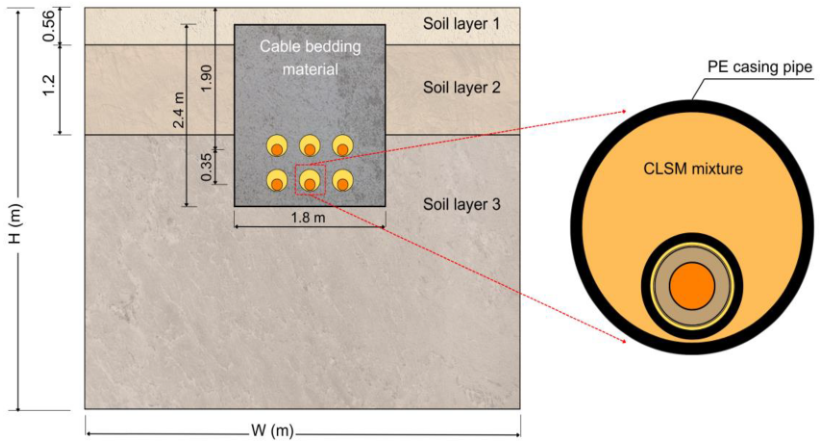
\includegraphics[width=\textwidth, keepaspectratio]{kim_fig01_upcs_geometry.png}\\
\refcite{\tiny Kim et al. (2025, p. 3), Fig. 1}

\column{0.57\textwidth}
\justifying\small
El sistema modelado corresponde a \textbf{6 cables de 154\,kV} en dos
capas horizontales (``two-flat formation'') dentro de un banco de ductos
enterrado hasta $H = 2{,}4$\,m de profundidad en Corea del Sur.

\vspace{0.5em}
\textbf{Capas del suelo identificadas:}
\begin{itemize}[leftmargin=*, itemsep=2pt]\scriptsize
  \item \textbf{Capa 1} (SC, arena arcillosa): $k_1 = 1{,}804$\,W/(m·K)
  \item \textbf{Capa 2} (CL, arcilla): $k_2 = 1{,}351$\,W/(m·K)
  \item \textbf{Capa 3} (CL, arcilla): $k_3 = 1{,}517$\,W/(m·K)
\end{itemize}

\vspace{0.4em}
\textbf{Entorno del cable:}
\begin{itemize}[leftmargin=*, itemsep=2pt]\scriptsize
  \item Tubo de casing de PE ($d_{cs}=220$\,mm)
  \item Relleno interior: mezcla CLSM (escoria de acero)
  \item \textit{Bedding} externo: arena / concreto normal / PAC
\end{itemize}

\vspace{0.4em}
\refcite{Kim et al. (2025, p. 3)}
\end{columns}
\end{frame}

\begin{frame}{Estructura interna del cable XLPE de 154\,kV }
\begin{columns}[T]
\column{0.48\textwidth}
\centering
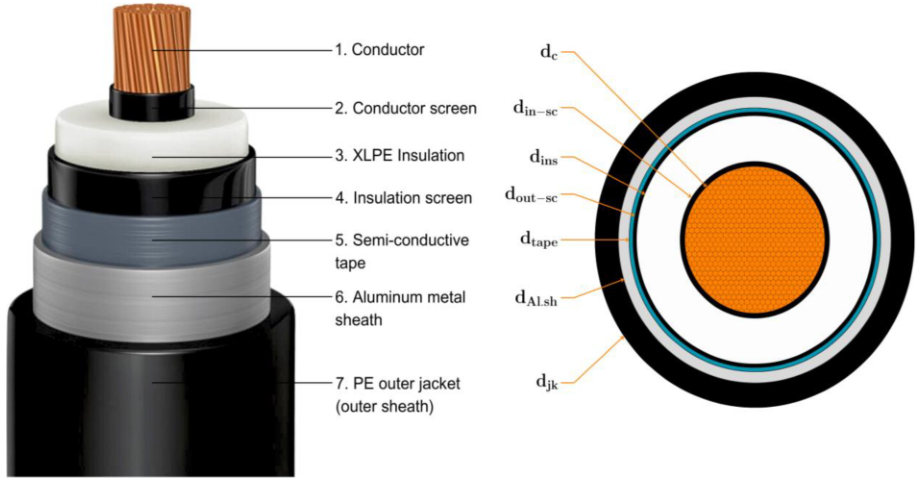
\includegraphics[width=\textwidth, keepaspectratio]{kim_fig02_cable_xsec.png}\\
\refcite{\tiny Kim et al. (2025, p. 4), Fig. 2}

\column{0.48\textwidth}
\small
\textbf{Capas del cable} (de adentro hacia afuera):

\vspace{0.4em}
\begin{tabular}{@{}lll@{}}
\toprule
\footnotesize Capa & \footnotesize Material & \footnotesize $k$ [W/(m·K)] \\
\midrule
\footnotesize Conductor & \footnotesize Cu & \footnotesize 400 \\
\footnotesize Screen cond. & \footnotesize XLPE & \footnotesize 0{,}286 \\
\footnotesize Aislamiento & \footnotesize XLPE & \footnotesize 0{,}286 \\
\footnotesize Screen aisla. & \footnotesize XLPE & \footnotesize 0{,}286 \\
\footnotesize Cinta semicon. & \footnotesize — & \footnotesize 0{,}167 \\
\footnotesize Vaina Al & \footnotesize Al & \footnotesize 237 \\
\footnotesize Chaqueta PE & \footnotesize PE & \footnotesize 0{,}286 \\
\footnotesize Casing PE & \footnotesize PE & \footnotesize 0{,}286 \\
\bottomrule
\end{tabular}

\vspace{0.5em}
\scriptsize
Diámetro total del casing: \textbf{220\,mm} ($t_{cs}=10$\,mm)\\
Conductor: $d_c = 42{,}4$\,mm (Cu)\\
Aislamiento XLPE: hasta $\varnothing\,80{,}4$\,mm

\vspace{0.4em}
\refcite{Kim et al. (2025, p. 4--5), Tab. 2}
\end{columns}
\end{frame}

% ===========================================================================
\section{Suelo heterogéneo y entorno del cable}
% ===========================================================================

\begin{frame}{Suelo heterogéneo: el problema físico real}
\begin{columns}[T]
\column{0.48\textwidth}
\begin{alertblock}{¿Por qué importa el suelo?}
\scriptsize\justifying
Más del \textbf{70\%} del aumento de temperatura del conductor se debe a
la resistencia térmica \textbf{externa} (el suelo y el relleno), no a las
capas del cable.
\refcite{(Kim et al., 2025, p. 2)}

El suelo es heterogéneo:
\begin{itemize}[leftmargin=*, itemsep=1pt]
  \item Distintas capas con $k$ diferente
  \item Variación estacional de la temperatura
  \item Secado térmico local bajo carga sostenida
  \item Variación vertical: estratos cambian con la profundidad.
\end{itemize}
\end{alertblock}

\vspace{0.1em}
\begin{block}{\small Propiedades de los 3 estratos (Tabla 6)}
\scriptsize
\begin{tabular}{@{}lccc@{}}
\toprule
Estrato & Clase. & $k$ [W/(m·K)] & $\rho$ [°C·cm/W]\\
\midrule
1 (SC) & Arena arcill. & 1,804 & 55,4 \\
2 (CL) & Arcilla & 1,351 & 74,0 \\
3 (CL) & Arcilla & 1,517 & 65,9 \\
\bottomrule
\end{tabular}\\
\tiny Medido con KD2 Pro (método aguja térmica lineal).\\
\refcite{Kim et al. (2025, p. 10), Tab. 6}
\end{block}

\column{0.48\textwidth}
\begin{exampleblock}{Temperatura del suelo: función $T(z,t)$}
\scriptsize\justifying
El paper adopta la solución analítica de Kusuda-Achenbach (1965) para la
temperatura del suelo en función de la profundidad $z$ y el tiempo $t$:
\[
T(z,t) = T_{\text{mean}} - A_s \, e^{-z\sqrt{\pi/(365\,D)}}
\cos\!\left[\frac{2\pi}{365}\!\left(t - t_0 - \frac{z}{2}\sqrt{\frac{365}{\pi D}}\right)\right]
\]
Donde $A_s$ es la amplitud anual superficial y $D$ la difusividad
térmica del suelo.
\end{exampleblock}

\vspace{0.1em}
\begin{block}{\small Implicación para la investigación}
\scriptsize
Los métodos IEC\,60287 usan temperaturas de referencia constante
\textbf{$T_{ref} = 20\,$°C}. El paper demuestra que las condiciones
reales de la instalación pueden diferir hasta \textbf{17,3\,°C} de ese supuesto.
\refcite{Kim et al. (2025, p. 14)}
\end{block}
\end{columns}
\end{frame}

\begin{frame}{Bedding: el material de relleno como variable de diseño}
\begin{columns}[T]
\column{0.44\textwidth}
\centering
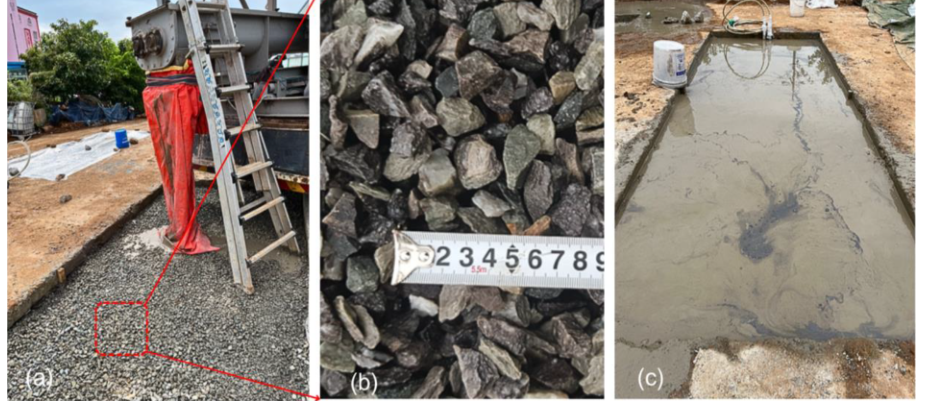
\includegraphics[width=\textwidth, keepaspectratio]{kim_fig12_PAC_construction.png}\\
\refcite{\tiny Kim et al. (2025, p. 11), Fig. 12: Construcción del PAC (2 etapas)}

\column{0.52\textwidth}
\small\justifying
El \textit{cable bedding material} o material de relleno rodea el banco
de ductos y define el camino térmico entre el cable y el suelo natural.

\vspace{0.4em}
\textbf{3 materiales comparados:}
\begin{itemize}[leftmargin=*, itemsep=3pt]\scriptsize
  \item \textbf{Arena (Sand)}: material convencional, $k=1{,}365$\,W/(m·K)
  \item \textbf{Concreto normal (NC)}: premezclado estándar,
        $k=2{,}093$\,W/(m·K) (+53\%)
  \item \textbf{PAC} (Prepacked Aggregate Concrete): concreto en dos
        etapas, áridos pre-colocados + lechada de alta fluidez,
        $k=2{,}094$\,W/(m·K) (+53\%)
\end{itemize}

\vspace{0.2em}
\begin{alertblock}{\small Ventaja del PAC}
\scriptsize
Igual conductividad que NC, pero \textbf{sin presión hidrostática}
sobre las tuberías de PE: más seguro en instalaciones profundas.
Permite usar agregados reciclados (concreto demolido, escoria).
\refcite{Kim et al. (2025, p. 21)}
\end{alertblock}
\end{columns}
\end{frame}

% ===========================================================================
\section{Problematica e hipótesis}
% ===========================================================================

\begin{frame}{Problematica: lo que fallan los métodos estándar}
\begin{columns}[T]
\column{0.4\textwidth}
\vspace{2.0em}
\begin{alertblock}{Supuestos de IEC\,60287 que no se cumplen en campo}
\scriptsize\justifying
\begin{itemize}[leftmargin=*, itemsep=2pt]
  \item Temperatura ambiente \textbf{constante} ($T_{ref}=20$°C)
  \item Conductividad del suelo \textbf{uniforme} ($k_s = \text{const}$)
  \item Carga de pérdidas al \textbf{100\%} del tiempo
  \item Efecto del aire superficial y radiación solar \textbf{ignorado}
  \item Superposición térmica de cables múltiples tratada de forma
        simplificada
\end{itemize}
\refcite{(Kim et al., 2025, p. 2); (IEC 60287-1-1, 2023)}
\end{alertblock}

\column{0.55\textwidth}
\begin{block}{Hipótesis del paper}
\small\justifying
\begin{enumerate}[leftmargin=*, itemsep=3pt]\scriptsize
  \item La ampacidad depende de las temperaturas
        \textbf{real} del ambiente y del suelo (no del valor de
        referencia 20°C).
  \item El material de \textit{bedding} con mayor conductividad
        térmica reduce la temperatura máxima del conductor de forma
        significativa.
  \item El FEM 2D con condiciones de contorno analíticas $T(z,t)$
        y $T_g$ reproduce con precisión el comportamiento térmico real.
\end{enumerate}
\refcite{Kim et al. (2025, p. 2)}
\end{block}

\vspace{0.4em}
\begin{exampleblock}{\small Conexión con nuestra investigación}
\scriptsize
El paper \textbf{establece el FEM como referencia de precisión} para el
campo 2D. Nuestra investigación propone reemplazar ese FEM por una PINN
que capture la física con menor costo computacional y permita resolver el
\textbf{problema inverso} ($k$ del suelo desde mediciones de temperatura).
\refcite{(Propuesta de investigación, MIA 2026-1)}
\end{exampleblock}
\end{columns}
\end{frame}

% ===========================================================================
\section{Metodología}
% ===========================================================================

\begin{frame}{Metodología (I): modelo analítico IEC\,60287}
\begin{columns}[T]
\column{0.58\textwidth}
\small\justifying
\textbf{Ecuación de ampacidad} (Neher-McGrath / IEC\,60287-1-1):
\[
I = \sqrt{\frac{\Delta T - W_d\left(\tfrac{1}{2}T_1 + n(T_2+T_3+T_4)\right)}
{R_{\text{AC}}\left(T_1 + n(1+\lambda_1)T_2 + n(1+\lambda_1+\lambda_2)(T_3+T_4)\right)}}
\]
\vspace{0.2em}
Donde $T_1$--$T_4$ son resistencias térmicas de las capas del cable y del
suelo; $W_d$ pérdidas dieléctricas; $R_{\text{AC}}$ resistencia del
conductor a CA.

\vspace{0.41em}
\textbf{Factor de pérdida de carga} $L_f$: El paper adopta el estándar
KEPCO DS-6210 de \textbf{80\%} en lugar del 100\% de IEC.
\refcite{Kim et al. (2025, p. 7--8)}

\vspace{0.3em}
\textbf{Temperatura del suelo en la frontera inferior:}
La función analítica de Kusuda--Achenbach (1965) da $T_g(z,t)$; se
impone como condición de Dirichlet en el borde inferior del dominio.
Ignorar $T_g$ genera error de \textbf{1,6°C en el conductor}.
\refcite{Kim et al. (2025, p. 14)}

\column{0.40\textwidth}
\begin{block}{\small Resistencia externa $R_4$ para banco de ductos}
\scriptsize
Múltiples cables generan \textbf{superposición térmica}. La resistencia
externa aumenta con el factor de pérdida:
\[
R_4 = \frac{\rho_b}{2\pi}\ln\frac{D_x}{d_{bc}} + \Delta T_{\text{mutual}}
\]

El factor de carga $L_f$ amplifica $R_4$ bajo condiciones reales de
operación.
\refcite{Kim et al. (2025, p. 8)}
\end{block}

\vspace{0.01em}
\begin{alertblock}{\small Limitación del modelo analítico}
\scriptsize
IEC\,60287 trata el suelo como \textbf{homogéneo} y usa $k_s$ promedio.
El paper muestra que las tres capas de suelo con $k$ diferente
no pueden reducirse a un solo valor sin error.
\refcite{Kim et al. (2025, p. 2)}
\end{alertblock}
\end{columns}
\end{frame}

\begin{frame}{Metodología (II): modelo numérico FEM (COMSOL)}
\begin{columns}[T]
\column{0.30\textwidth}
\centering
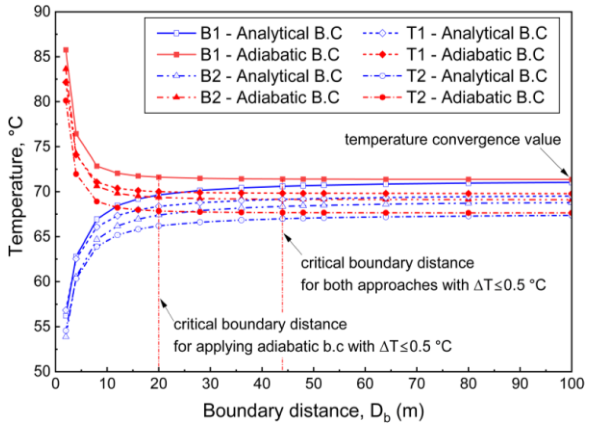
\includegraphics[width=0.85\textwidth, keepaspectratio]{kim_fig08_domain_boundary.png}\\
{\tiny \refcite{Kim et al. (2025, p. 9), Fig. 8: Convergencia vs. distancia $D_b$}}

\vspace{0.3em}
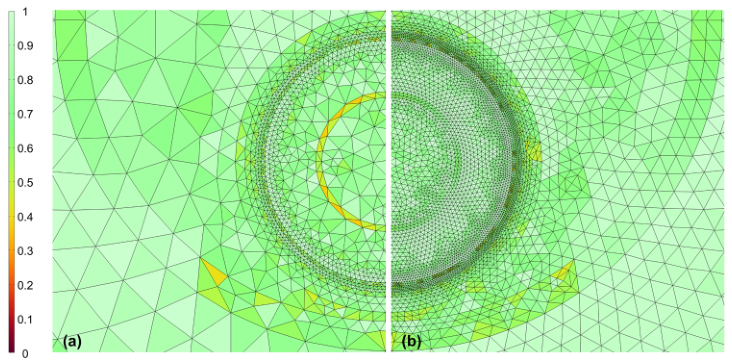
\includegraphics[width=0.85\textwidth, keepaspectratio]{kim_fig09_mesh_quality.png}\\
{\tiny \refcite{Kim et al. (2025, p. 9), Fig. 9: Calidad del mallado}}

\column{0.66\textwidth}
\small
\textbf{Modelo FEM 2D estacionario} (COMSOL Multiphysics v6.1):
\[
\frac{\partial}{\partial x}\!\left(k\frac{\partial T}{\partial x}\right)
+ \frac{\partial}{\partial y}\!\left(k\frac{\partial T}{\partial y}\right)
+ \dot{q} = 0
\]

\vspace{0.3em}
\textbf{Independencia del mallado:}
\begin{itemize}[leftmargin=*, itemsep=1pt]\scriptsize
  \item Malla automática (16\,629 nodos): $T_{c,\text{max}}=70{,}606$°C
  \item 1era. refinación (66\,326 nodos): $\Delta T = 0{,}001$°C
  \item Se usa 1era. refinación como solución definitiva
\end{itemize}
\refcite{Kim et al. (2025, p. 9), Tab. 4}

\vspace{0.3em}
\textbf{Condiciones de contorno:}
\begin{itemize}[leftmargin=*, itemsep=1pt]\scriptsize
  \item \textbf{Superior}: convección natural/forzada (coef. $h$,
        función de $T_{\text{amb-air}}$ y viento Gwangju)
  \item \textbf{Inferior}: Dirichlet $T_g(z,t)$ — función analítica
  \item \textbf{Laterales}: Neumann $\nabla T=0$ (adiabáticas)
  \item \textbf{Cables}: fuente de calor $\dot{q} = I^2 R_{AC}/(A_c)$
\end{itemize}
\refcite{Kim et al. (2025, p. 6--7)}
\end{columns}
\end{frame}

% ===========================================================================
\section{Resultados}
% ===========================================================================

\begin{frame}{Resultados (I): ampacidad crítica estacional (Fig. 17)}
\centering
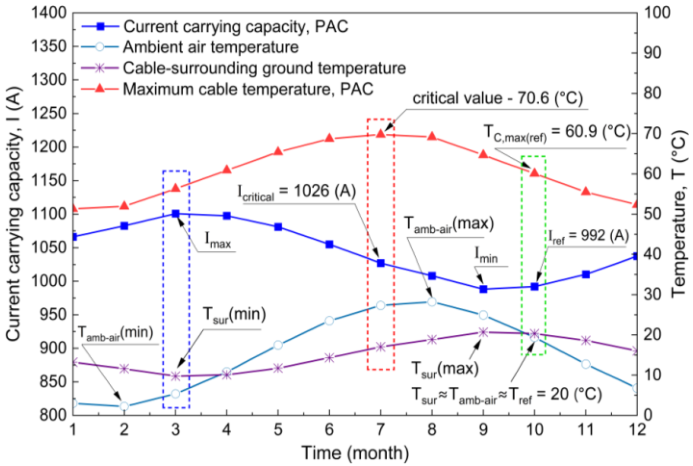
\includegraphics[width=0.7\textwidth, keepaspectratio]{kim_fig17_ccc_seasonal.png}\\
\refcite{\tiny Kim et al. (2025, p. 14), Fig. 17: Temperatura máx. del cable vs. ampacidad y temperatura del suelo — evolución mensual}

\vspace{0.3em}
\begin{columns}[T]
\column{0.48\textwidth}
\scriptsize
\begin{itemize}[leftmargin=*, itemsep=2pt]
  \item La ampacidad \textbf{mínima} ocurre en \textbf{julio} (caso 5):
        $I_{crítico}=1026$\,A, $T_{c,max}=70{,}6$°C
        (\textit{caso de diseño})
  \item La ampacidad \textbf{máxima} se da en enero:
        $I_{max}=1350$\,A aprox.
  \item El mínimo de ampacidad ocurre en \textbf{septiembre},
        no en agosto, por el retardo de difusión del calor en el suelo
\end{itemize}
\column{0.48\textwidth}
\scriptsize
\begin{itemize}[leftmargin=*, itemsep=2pt]
  \item Con $T_{ref}=20$°C (referencia IEC): $I_{ref}=992$\,A y
        $T_{c,max}=60{,}9$°C — \textbf{subestima} el calentamiento real
  \item En octubre $T_{sur} \approx T_{amb} \approx 20$°C,
        lo que confirma la representatividad del caso de referencia solo
        para ese mes
  \item \textbf{Conclusión}: la ampacidad real varía hasta $\pm 30\%$
        respecto al valor estático estándar durante el año
\end{itemize}
\end{columns}
\end{frame}

\begin{frame}{Resultados (II): contornos de temperatura — arena vs. PAC}
\begin{columns}[T]
\column{0.52\textwidth}
\centering
\small\textbf{Concreto Normal (NC)} — Verano e invierno\\[0.3em]
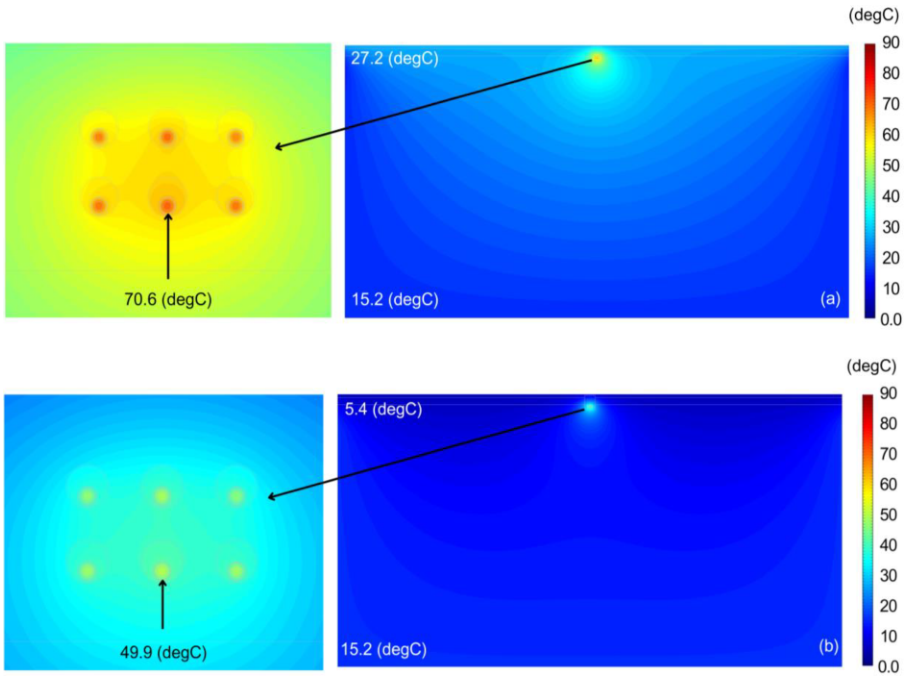
\includegraphics[width=0.72\textwidth, keepaspectratio]{kim_fig20_NC_contour.png}\\
\refcite{\tiny Kim et al. (2025, p. 16), Fig. 20}

\column{0.52\textwidth}
\centering
\small\textbf{PAC} — Verano e invierno\\[0.3em]
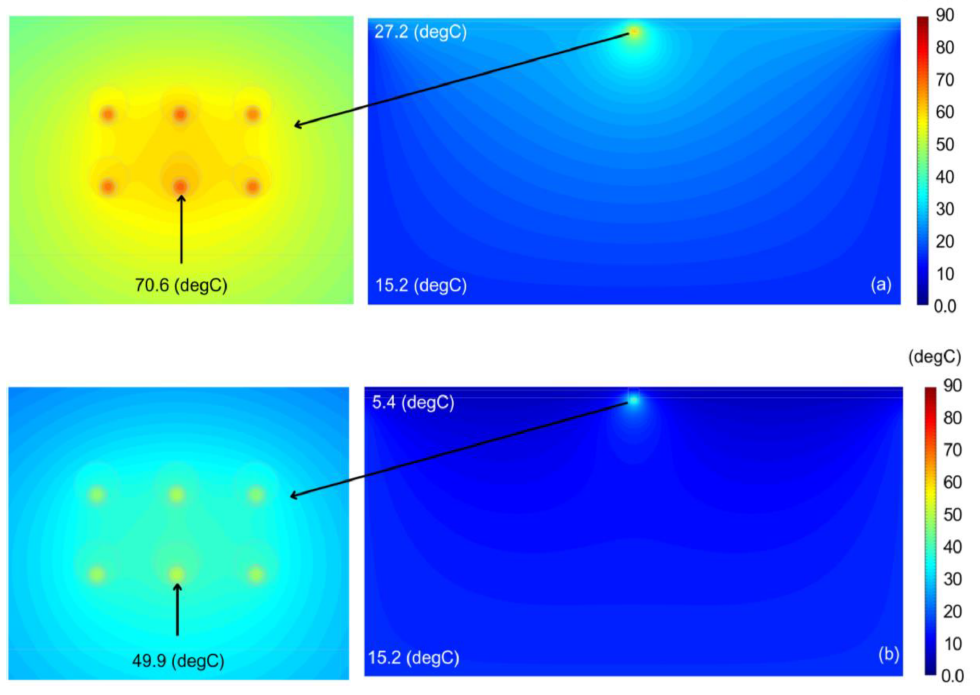
\includegraphics[width=0.75\textwidth, keepaspectratio]{kim_fig21_PAC_contour.png}\\
\refcite{\tiny Kim et al. (2025, p. 17), Fig. 21}
\end{columns}

\vspace{0.7em}
\begin{columns}[T]
\column{0.50\textwidth}
\scriptsize
NC y PAC tienen conductividades prácticamente iguales
($k \approx 2{,}094$\,W/(m·K)); los contornos son idénticos.
El campo térmico 2D muestra la \textbf{zona de mayor gradiente} alrededor
del banco de ductos dentro del \textit{bedding}.
\column{0.52\textwidth}
\scriptsize
Temperatura máx. en verano: \textbf{70,6°C} (PAC/NC) vs.
\textbf{77,6°C} (arena). \\ Temperatura máx. en invierno: \textbf{49,9°C}
(PAC/NC) vs. \textbf{57,1°C} (arena). \\
Diferencia: \textbf{$\approx 7$°C} en favor de PAC.
\refcite{Kim et al. (2025, p. 16)}
\end{columns}
\end{frame}

\begin{frame}{Resultados (III): comparación de perfiles — Fig. 25}
\centering
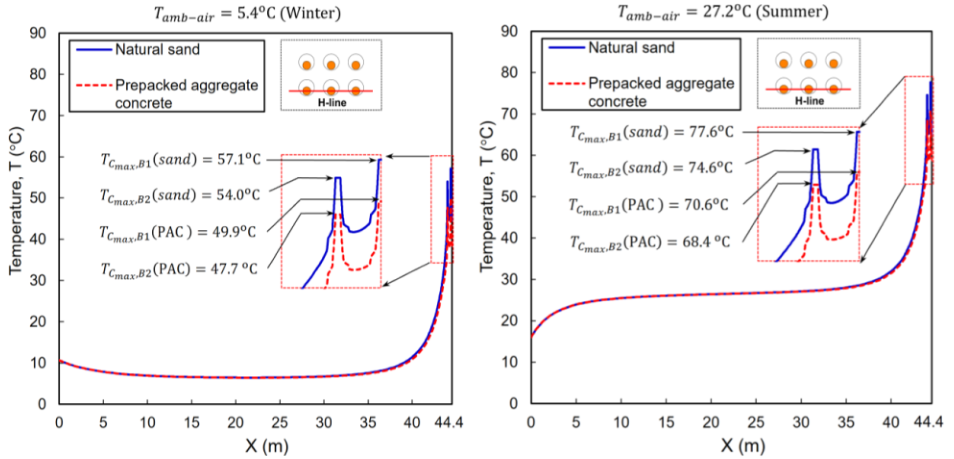
\includegraphics[width=0.57\textwidth, keepaspectratio]{kim_fig25_comparison.png}\\
\refcite{\tiny Kim et al. (2025, p. 21), Fig. 25: Perfil de temperatura horizontal para arena vs. PAC — invierno y verano}

\vspace{0.28em}
\begin{columns}[T]
\column{0.3\textwidth}
\scriptsize
\begin{tabular}{@{}lcc@{}}
\toprule
 & \textbf{Verano} & \textbf{Invierno}\\
\midrule
Arena $T_{c,B1}$ & 77,6°C & 57,1°C \\
Arena $T_{c,B2}$ & 74,6°C & 54,0°C \\
PAC $T_{c,B1}$ & \textbf{70,6°C} & \textbf{49,9°C} \\
PAC $T_{c,B2}$ & \textbf{68,4°C} & \textbf{47,7°C} \\
\bottomrule
\end{tabular}\\[0.2em]
Diferencia PAC/arena: \textbf{7,0°C en verano}, \textbf{7,2°C en invierno}

\column{0.71\textwidth}
\scriptsize
\begin{itemize}[leftmargin=*, itemsep=2pt]
  \item PAC \textbf{reduce el punto caliente} del cable más expuesto
        (B1, capa superior) en $\approx 7$°C
  \item Con límite térmico XLPE de 90°C, esto \textbf{amplía el margen}
        de seguridad de 12,4°C a 19,4°C
  \item O bien permite aumentar la ampacidad (más carga para igual margen)
  \item El perfil horizontal confirma el gradiente concentrado en el
        \textit{bedding} y su dependencia de $k$ del relleno
\end{itemize}
\end{columns}
\end{frame}

% ===========================================================================
\section{Aportes, límites y ventaja PINN}
% ===========================================================================

\begin{frame}{Aportes del paper a nuestra investigación}
\begin{columns}[T]
\column{0.53\textwidth}
\begin{exampleblock}{Lo que el paper aporta}
\small\justifying
\begin{itemize}[leftmargin=*, itemsep=3pt]
  \item \textbf{Geometría y datos de referencia}: cable 154\,kV, 6
        conductores en banco de ductos con suelo real de 3 capas
        $\Rightarrow$ caso \textit{benchmark} para validar nuestra PINN
  \item \textbf{Valores numéricos precisos}: $T_{c,max}=70{,}6$°C para
        PAC, $77{,}6$°C para arena.
  \item \textbf{Condiciones reales}: temperatura estacional, $k$ medido,
        factor de carga KEPCO 80\%
  \item \textbf{Metodología reproducible}: COMSOL + IEC\,60287 bien
        documentados
  \item \textbf{Justificación del problema}: demuestra cuantitativamente
        que ignorar las condiciones reales genera errores de $>7$°C
\end{itemize}
\refcite{Kim et al. (2025, pp. 14--21)}
\end{exampleblock}

\column{0.43\textwidth}
\begin{alertblock}{Limitaciones del paper}
\small\justifying
\begin{itemize}[leftmargin=*, itemsep=3pt]
  \item Solo \textbf{régimen estacionario}: no captura transitorios ni
        DTR (calificación dinámica)
  \item \textbf{FEM requiere re-mallado} para cada geometría o
        configuración nueva
  \item Sin \textbf{problema inverso}: no estima $k$ del suelo desde
        temperatura medida
  \item Alta barrera de acceso: licencia COMSOL, configuración experta
  \item No integrable en tiempo real con SCADA u otros sistemas
        operacionales
\end{itemize}
\refcite{Kim et al. (2025, p. 21); CIGRÉ WG B1.56 (2022)}
\end{alertblock}
\end{columns}
\end{frame}

\begin{frame}{¿Por qué una PINN supera estas limitaciones? (muy breve)}
\begin{columns}[T]
\column{0.52\textwidth}
\begin{exampleblock}{Ventajas de una PINN sobre el FEM del paper}
\small
\begin{itemize}[leftmargin=*, itemsep=4pt]
  \item \textbf{Sin remallado}: la red aprende el operador físico y
        generaliza a nuevas geometrías y materiales
  \item \textbf{Problema inverso} natural: puede estimar $k(x,y)$ desde
        observaciones de temperatura operativa
  \item \textbf{Transitorio} sin costo adicional: añadir la derivada
        temporal $\partial T/\partial t$ es directo
  \item \textbf{Integración operacional}: una vez entrenada, la red
        evalúa en milisegundos $\Rightarrow$ DTR en tiempo real
  \item \textbf{Open-source}: PyTorch / JAX, reproducible
\end{itemize}
\end{exampleblock}

\column{0.44\textwidth}
\begin{block}{\small Brecha de investigación identificada}
\small\justifying
El paper \textbf{Kim et al. (2025)} demuestra que el FEM 2D es la
herramienta correcta para el problema, pero no aborda:

\vspace{0.3em}
\begin{itemize}[leftmargin=*, itemsep=2pt]\scriptsize
  \item Operación dinámica / DTR
  \item Estimación inversa de $k$
  \item Geometrías variables sin re-mallado
  \item Integración con sensores operativos
\end{itemize}

\vspace{0.3em}
\textbf{Nuestra propuesta}: reemplazar el FEM estacionario por una PINN
entrenada sobre la física de la ecuación de Fourier 2D con $k(x,y)$
variable, usando el caso Kim\,2025 como \textit{benchmark} de validación.
\refcite{(Propuesta MIA 2026-1)}
\end{block}
\end{columns}
\end{frame}

% ===========================================================================
\section{Conclusiones}
% ===========================================================================

\begin{frame}{Síntesis del paper y conexión con el problema de investigación}
\begin{columns}[T]
\column{0.48\textwidth}
\begin{block}{\small Conclusiones del paper (Kim et al., 2025)}
\scriptsize\justifying
\begin{enumerate}[leftmargin=*, itemsep=2pt]
  \item[(i)] La ampacidad es función de las temperaturas reales del
        ambiente; el valor de referencia 20°C es válido solo en octubre
        (Corea del Sur).
  \item[(ii)] Usar la función analítica $T(z,t)$ como condición inferior
        reduce el error en el conductor en 1,6°C y en el fondo del dominio
        en 14,5°C.
  \item[(iii)] PAC ($k = 2{,}094$\,W/(m·K)) reduce la temperatura máxima
        del conductor de 77,6°C (arena) a 70,6°C en verano.
  \item[(iv)] PAC usa agregados reciclados; posible alternativa
        económica y ambiental al concreto convencional.
\end{enumerate}
\refcite{Kim et al. (2025, p. 21)}
\end{block}

\column{0.48\textwidth}
\begin{exampleblock}{\small Impacto en nuestra investigación}
\scriptsize\justifying
\begin{itemize}[leftmargin=*, itemsep=3pt]
  \item \textbf{El caso Kim\,2025 es el benchmark principal} de
        validación del modelo PINN que desarrollaremos
  \item Confirma que el suelo heterogéneo y las condiciones estacionales
        generan diferencias de $>7$°C en el conductor: la brecha es real
        y cuantificada
  \item El dato $T_{c,max}=70{,}6$°C (PAC, julio) es nuestra
        \textbf{meta de precisión} ($\pm 1$°C)
  \item Los datos de materiales (Tablas 5, 6, 9) son insumo directo
        para el dominio físico de la PINN
  \item Los límites del FEM justifican la propuesta: PINN para DTR,
        problema inverso y generalización geométrica
\end{itemize}
\refcite{(Propuesta de Investigación, MIA 2026-1, Luis Koc \& Herbert Meléndez)}
\end{exampleblock}
\end{columns}
\end{frame}

% ===========================================================================
\section{Referencias}
% ===========================================================================

\begin{frame}[allowframebreaks]{Referencias}
\footnotesize
\textbf{Paper reseñado:}
\begin{itemize}[leftmargin=*]
  \item Kim, Y.-S., Nguyen Cong, H., Dinh, B.\,H., \& Kim, H.-K.
        (2025). \textit{Effect of ambient air and ground temperatures on
        heat transfer in underground power cable system buried in newly
        developed cable bedding material}. \textbf{Geothermics}, 125,
        103151. \url{https://doi.org/10.1016/j.geothermics.2024.103151}
\end{itemize}

\vspace{0.5em}
\textbf{Normas y estándares citados:}
\begin{itemize}[leftmargin=*]
  \item IEC 60287-1-1 (2023). \textit{Electric cables --- Calculation of
        the current rating --- Part 1-1: Current rating equations
        (100\% load factor) and calculation of losses}. IEC.
  \item IEC 60287-2-1 (2023). \textit{Electric cables --- Calculation of
        the current rating --- Part 2-1: Thermal resistance}. IEC.
  \item Neher, J.\,H., \& McGrath, M.\,H. (1957). The calculation of
        the temperature rise and load capability of cable systems.
        \textit{AIEE Trans.}, 76(3), 752--772.
\end{itemize}

\vspace{0.5em}
\textbf{Otras referencias utilizadas:}
\begin{itemize}[leftmargin=*]
  \item Anders, G.\,J. (2005). \textit{Rating of Electric Power Cables
        in Unfavorable Thermal Environments}. IEEE Press/Wiley.
  \item Kusuda, T., \& Achenbach, P.\,R. (1965). Earth temperature and
        thermal diffusivity at selected stations in the United States.
        \textit{ASHRAE Trans.}, 71(1), 61--75.
  \item Aras, F., Oysu, C., \& Yilmaz, G. (2005). An assessment of
        the methods for calculating ampacity of underground power cables.
        \textit{Electric Power Components and Systems}, 33(12), 1385--1402.
  \item CIGRÉ WG B1.56 (2022). \textit{Cable Rating Considering
        Non-Uniform Soil Thermal Resistivity}. CIGRÉ.
  \item Dinh, B.\,H., et al. (2020). CLSM with steelmaking slag.
        (Referenciado en Kim et al., 2025, p. 10.)
  \item Propuesta de Investigación MIA 2026-1. Luis Koc \& Herbert
        Meléndez. \textit{Trabajo de Investigación I} --- Grupo G91,
        Universidad Nacional de Ingeniería, 2026.
\end{itemize}
\end{frame}

% ===========================================================================
\end{document}
% ===========================================================================
